\documentclass{beamer} % Gliederung im Kopf, sections und subsections
\setbeamertemplate{navigation symbols}{}%remove navigation symbols

\usepackage{tikz}
\usetikzlibrary{shapes,arrows,positioning,chains,fit,calc,matrix,decorations.pathreplacing}
\usepackage{xcolor}\usepackage{subfloat}\usepackage{subfig}

\usetikzlibrary{intersections}


\usepackage{tikz}
\usetikzlibrary{arrows,decorations.pathmorphing,backgrounds,positioning,fit,petri}
\renewcommand*{\familydefault}{\sfdefault}

\tikzset{forestyle/.style = {rectangle, thick, minimum width = 5cm, minimum height = 0.5cm, text width = 4.5cm, outer sep = 1mm},
  pre/.style={<-, shorten <=1pt, >=stealth, ultra thick},
  extend/.style={<-,dashed, shorten <=1pt, >=stealth, ultra thick}}



\def\firstcircle{[name path=firstcircle] (0,0) circle (3cm)}
\def\secondcircle{[name path=secondcircle] (55:3.11111cm) circle (3cm)} %No idea how the numbers selected work; they were derived from what I found online. They seem to function though!
\def\thirdcircle{[name path=thirdcircle] (0:3.5cm) circle (3cm)}


\mode<presentation>

\begin{document}

\begin{frame}
\begin{center}
\begin{figure}[h!]\centering
\captionsetup[subfigure]{labelformat=empty}

\subfloat[Absent]{
\scalebox{0.15}{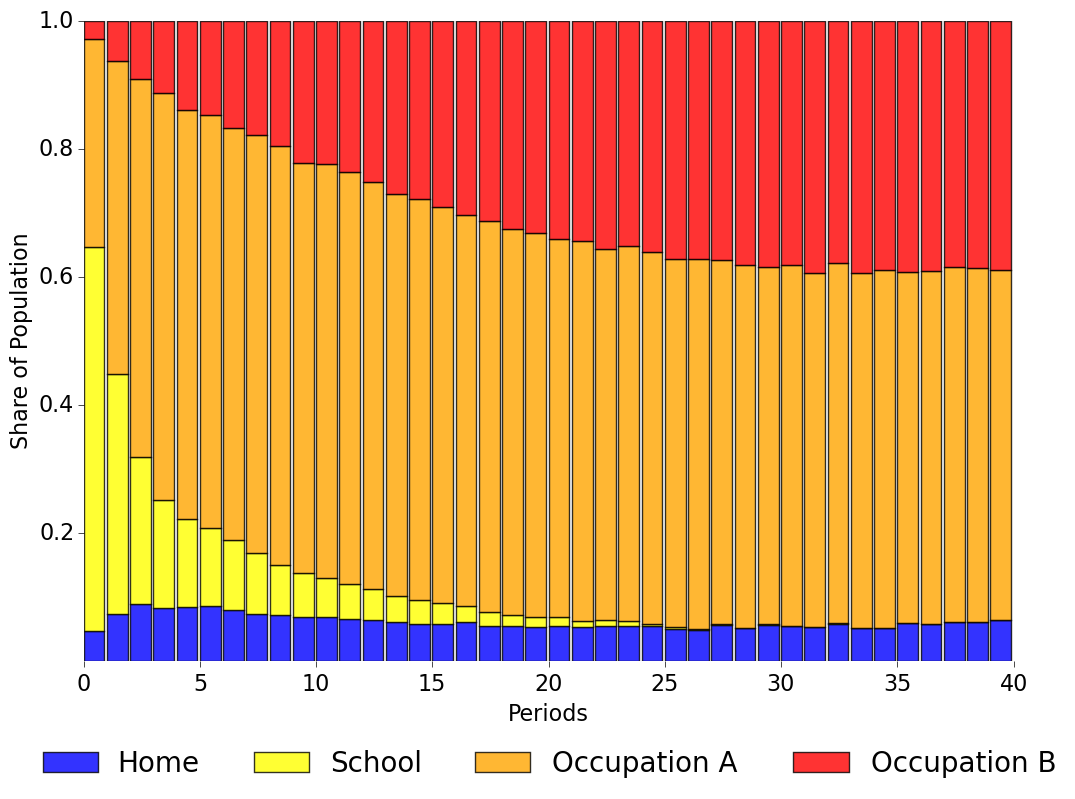
\includegraphics{choice_patterns_0000}}}\\\vspace{-0.1cm}
\subfloat[Low]{\
\scalebox{0.15}{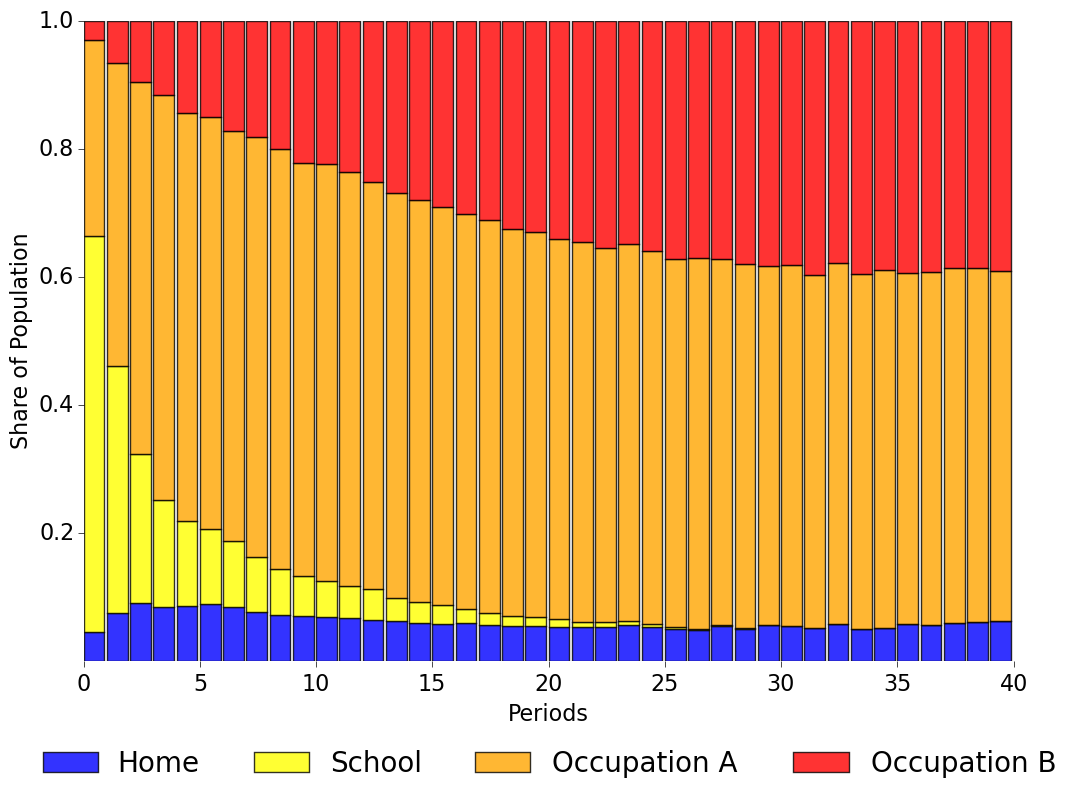
\includegraphics{choice_patterns_0033}}}\hspace{1.0cm}
\subfloat[High]{\
\scalebox{0.15}{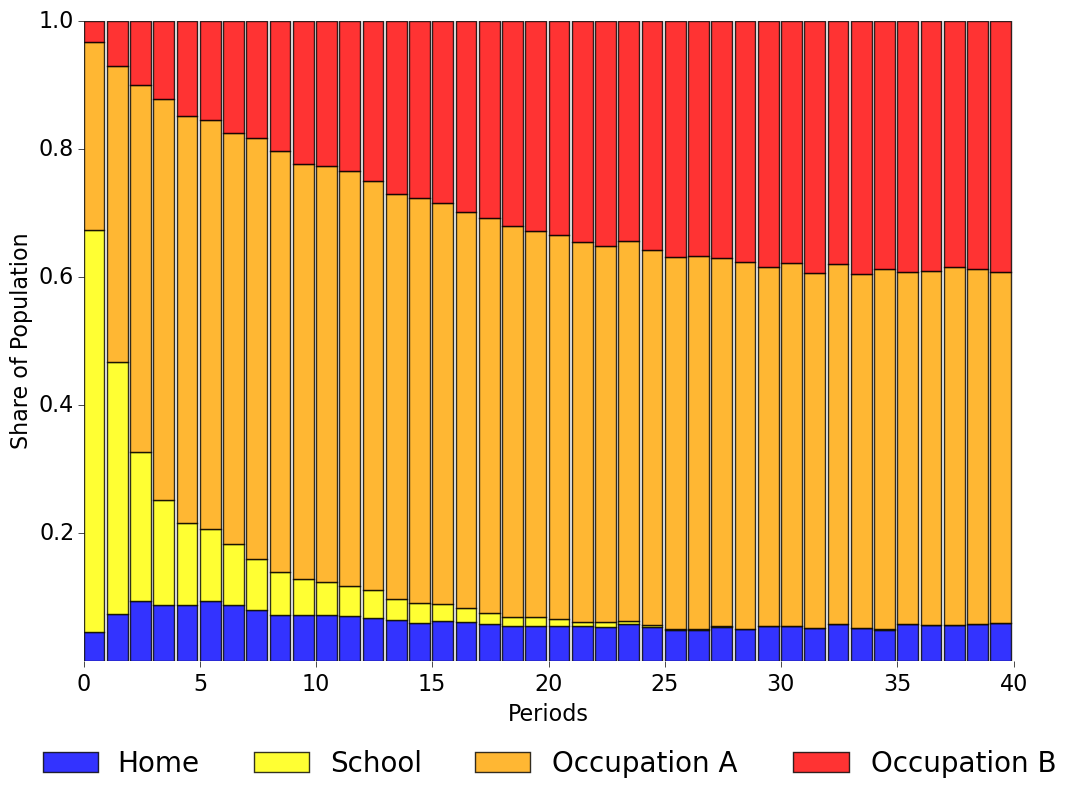
\includegraphics{choice_patterns_0142}}}
\end{figure}\end{center}\end{frame}
\end{document}
